\section{Adoption Focused Platforms} \label{chapter3:software-abstraction}

Section \ref{chapter3:software-productivity} and section \ref{chapter3:software-efficiency} present the platforms focusing respectively on productivity and efficiency, and conclude that favoring on one negatively impacts the other.
Moreover, a balance between productivity and efficiency is required to be both supported by the community and needed by the industry, hence trigger a virtuous circle of adoption.
This section presents platforms featuring an abstraction of the tasks organization to allow developers to focus on the modular organization to keep both productivity and efficiency.
Section \ref{chap3:software-abstraction:compilers} presents Compilers, and section \ref{chap3:software-abstraction:runtimes} presents Runtimes.

% \nt{read and include \cite{Catanzaro2009} it is about Productivity language JIT compilation into efficient language
% And get all the paper that cite this one.}
% \nt{read and include \cite{Engler1994}}
% \nt{read and include \cite{Kovachev2011}}
% \nt{read and include \cite{Asanovic2006}}

\begin{figure}[!h]
\begin{center}
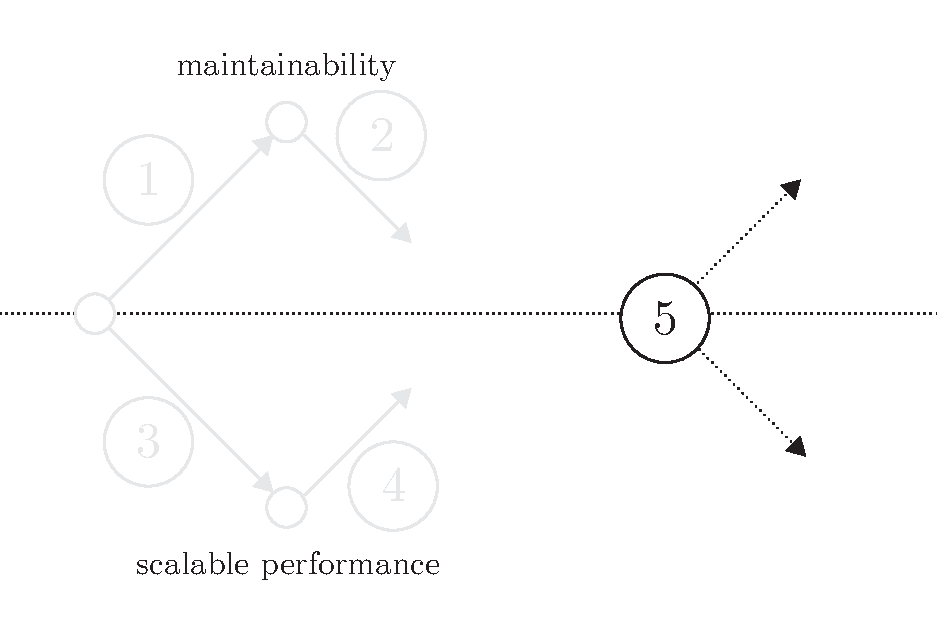
\includegraphics[width=0.6\textwidth]{../ressources/state-of-the-art-5.pdf}
\end{center}
\caption{Focus on Adoption}
\label{fig:state-of-the-art-5}
\end{figure}

\subsection{Abstraction of Tasks Organization}

\subsubsection{Compilers} \label{chapter3:software-abstraction:compilers}

\cit{It is a mistake to attempt high concurrency without help from the compiler}{R. Behren, J. Condit, E. Brewer \cite{Behren2003}}.

As soon as the incompatibility between the modules and the tasks organizations were presented, it was suggested to use a compilation approach to mitigate this incompatibility \cite{Parnas1972}.
% When showing the incompatibility between the two organization, D. Parnas  advocated conciliating the two methods using an assembler to transform the development organization into the execution organization \cite{Parnas1972}.
This section presents the state of the art to extract parallelization from sequential programs through code transformation and compilation.

\nt{read and include \cite{Catanzaro2009}}

\paragraph{Parallelism Extraction}

Extracting parallelism from a sequential implementation is a hard problem \cite{Johnston2004a}.
A compiler needs to identify the commutative operations to parallelize their executions \cite{Rinard1996,Clements2013a}.

An important work was done to parallelize loop iterations \cite{Mauras1989,Amarasinghe1995,Chen2008,Banerjee2013,Radoi2014}, particularly using the polyhedral compilation method \cite{Bastoul2004}.
Examples of polyhedral compilers are \ImplementationsOf{Polyhedral Compilers}.
To improve performance gains outside of loops, some compilers identify the data-flow parallelism on the whole program \cite{Beck1991,Catanzaro2009,Li2012}.
Moreover, the data-flow representation and execution of a program is well suited for modern data processing applications \cite{Fernandez2014a}, as well as web services \cite{Salmito2013}.
% \nt{TODO Extract parallelism compilers from these :
% Load balanced pipeline parallelism \cite{Kamruzzaman2013}, 
% Regent \cite{Slaughter2015},
% Cilk-P, On-the-Fly Pipeline Parallelism\cite{Lee2013}
% }

% However, the limitation of modular programming regarding parallelization persists.
% In a purely functional language with immutability, higher-order functions are referentially transparent which implies commutativity hence parallelism \nt{Add reference of parallel purely functional languages}.
% \cite{Herrmann2000}
Mutable closures required for higher-order programming remains a challenge to parallelize because of the memory references shared across the program \cite{Harrison1989, Nicolay2010, Matsakis2012a}.
The next paragraphs present some improvements in compilation applicable for parallelism extraction.
% The first paragraph presents static analysis, while the second presents annotations systems.

% - Continuation-passing style parallelization compilation \cite{Harrison1989}.The interprocedural analysis and automatic parallelization of Scheme programs
% - Automatic Parallelization of Scheme Programs using Static Analysis \cite{Nicolay2010}

% - Commutativity analysis: A new analysis framework for parallelizing compilers \cite{Rinard1996}
% In this paper, they analyze commutative operations to parallelize them.
% It is novel because it isn't about parallelizing loops.
% However, it is not exactly pipeline parallelism either.

% Introducing 'Bones': a parallelizing source-to-source compiler based on algorithmic skeletons \cite{Nugteren2012}

\paragraph{Static analysis}

Compilers statically analyze the control-flow of a program to detect commutative operations \cite{Allen1970}.
The point-to analysis identifies side-effects \cite{Andersen1994,Jang2009,Sridharan2012,Wei2014} which allows to infer commutativity.
However, this analysis is not sufficient to track the dynamic control-flow of higher-order functions \cite{Shivers1991} like used in Javascript.

Another approach, abstract interpretation, is to interpret the possible path of executions.
It allows to statically reason on the behavior of dynamic program \cite{Maffeis2008,Smith2011,Gardner2012,Hackett2012,Raychev2013,Gardner2013,Bodin2014}.
It is successfully used for security applications \cite{Huang2004,Jovanovic2006,Yu2007,Maffeis2009a,Chudnov2015,Dolby2015}\nt{Update the citation for Dolby2015}.

However, these static analysis techniques remains often too imprecise, and expensive for the performance gain to be profitable.
Instead, some compilers relies on annotations from the developers.

\paragraph{Annotations}

Some works proposed to rely on annotations from the developer to identify the shared data structures and infer the commutativity of operations \cite{Vandierendonck2010a,Fernandez2014a}.
Such annotations are especially relevant for accelerators such as GPUs or FPGAs, because the development effort yields huge performance improvements \cite{Tarditi2006}.
Examples of such compilers are \ImplementationsOf{Annotation Compiler}.

% Bloom declarative language \ftnt{http://bloom-lang.net/}
% Blazes: Coordination analysis for distributed programs \cite{Alvaro2014}

% Livescript
% Typescript 
% Annotations, but not for parallelism.
% Asynchronism annotations should be sufficient.

\paragraph{Compilation Limitations}

% The static analysis of low level languages like Fortran or C, brings performance improvements.
For dynamic, higher-level languages like Javascript, the static analysis is not sufficient to correctly infer the independence of operations to parallelize them.
And parallel compilers often fall back on relying on annotation provided by developers.
Hence, the burden of detailing the tasks organization falls back to the developer, similarly to the platforms presented in the previous section.

Alternatively, another approach is to rely on the runtime to detect and distribute the commutative operations, and assure the communications.
The next paragraphs present runtime allowing this dynamic distribution.

\subsubsection{Runtimes} \label{chapter3:software-abstraction:runtimes}

\paragraph{Partitioned Global Address Space}

The Partitioned Global Address Space (PGAS) provides a uniform memory access on a distributed architecture.
It attempts to combine the efficiency of distributed memory systems, with the productivity of shared memory systems.
Each computing node executes the same program, and provide its local memory to be shared with all the other nodes.
The PGAS platform assures the remote accesses and synchronization of memory across nodes.
Examples of implementation of the PGAS model are \ImplementationsOf{Partitioned Global Address Space}.

\paragraph{Dynamic Distribution of Execution}

% It follows the PCAM design methodology \cite{Foster1995} to 
Following SEDA, Leda proposes a model where the independent stages of the pipeline are defined only by their role in the application \cite{Salmito2013,Salmito2014}.
% Partition $\to$ Communicate $\to$ Agglomerate $\to$ Map.
The execution distribution and module organization are different.
The actual execution distribution is defined automatically during deployment. % , only after the development
% blurs the distinction between the parallel organization of execution, and the modular organization of implementation.
This automation manages the execution organizations to help the developer focus on the modular organization.
However, it doesn't improve the composition of module with higher-order programming.

\paragraph{}

Tables \ref{tab:abstraction-maintainability} and \ref{tab:abstraction-performance} presents the platforms presented in this section regarding maintainability and performance.

\AbstractionProductivityTable{tab:abstraction-maintainability}

\AbstractionEfficiencyTable{tab:abstraction-performance}



\subsection{Adoption Limitations}

All the platforms presented in this section come from the need of the industry to reduce the development commitment required for efficiency.
However, these platforms are limited to scientific applications.
They respond exclusively to academic or industrial needs, and are barely supported by the community.

The balance between efficiency and productivity is not sufficient for a community of passionate to gather around the platform.
The platforms need to answer to needs of small scale for novice to start learning, and to incite the community to experiment and start projects organically.
The context of web development is particularly adapted for this requirement.

\AbstractionAdoptionTable{tab:abstraction-performance}

\subsection{Summary}

Table \ref{tab:abstraction-summary} summarizes the characteristics of the platforms presented in this section.

\AbstractionSummaryTable{tab:abstraction-summary}

\endinput
























\section{Due Related works} \label{section:related}

To our knowledge, our work is the first to explore the transformation from continuations to Promises in Javascript, and to state the similarity between Promises and data-flow programming.
This section presents the various works related to ours.
Our work is based on the previous work on Promises and Futures~\cite{Liskov1988}, and their specifications in Javascript\footnote{\url{https://promisesaplus.com/}}\footnote{\url{https://people.mozilla.org/~jorendorff/es6-draft.html\#sec-promise-objects}}.


Because of its dominant position in the web, Javascript is recently subject to a growing interest in the field of static analysis.
We identify two teams working on static analysis for Javascript.
In the Department of Computing, Imperial College London, S. Maffeis, P. Gardner and G. Smith realised a large body of work around the static analysis of Javascript.
Their work is based around an operational semantic~\cite{Maffeis2008} to bring program understanding~\cite{Smith2011,Gardner2012,Gardner2013,Bodin2014}.
Their goal seems to revolve around security applications of this analysis~\cite{Maffeis2009,Maffeis2009a}.
In a collaboration between the programming language research groups at Aarhus University and Universität Freiburg, P. Thiemann, S. Jensen and A. Møller are working on the static analysis of Javascript.
They presented a tool providing type inference using abstract interpretation~\cite{Thiemann2005,Jensen2009,Jensen2012}.
Their goal is to improve the tools available for Javascript developers~\cite{Andreasen}.
Another example of interest for Javascript static analysis is the adaptation of the points-to analysis from L. Andersen's thesis~\cite{Andersen1994} to Javascript, by D. Jang \textit{et al.}~\cite{Jang2009} and S. Wei \textit{et al.}~\cite{Wei2014}.

The industry seems to follow the same trends.
There are some security tools based on static analysis.
We can cite for example, the company Shape Security\footnote{\url{https://shapesecurity.com/}}.
They developed \textit{Esprima}, a Javascript parser, and a serie of tools to help static analysis.
Facebook released flow\footnote{\url{http://flowtype.org/}} on 26 October 2014, a static type checker for Javascript.

Promises combine controls over the execution and the data flow.
It arrange the execution parts sequentialy and assign the result of one into the inputs of the next.
This arrangement seems similar to some works on the field of functional and data-flow programming~\cite{Johnston2004,Cohen2012,Morrison1994,Kahn1974}.
We consider it a first step in the merge of elements from the data-flow paradigm into the imperative paradigm.
The Functional Reactive Programming paradigm pushes the intrication of data and control-flow even further~\cite{Winograd-Cort2013}.
